\section{Описание и исходные данные}
Команда разработчиков из 16 человек занимается созданием карты города на основе собственного модуля отображения. 
Проект должен быть завершен в течение 6 месяцев. 
Бюджет проекта: 50000 рублей.

\subsection{Исходнй план выполения задач}
\begin{figure}[H]
	\centering
	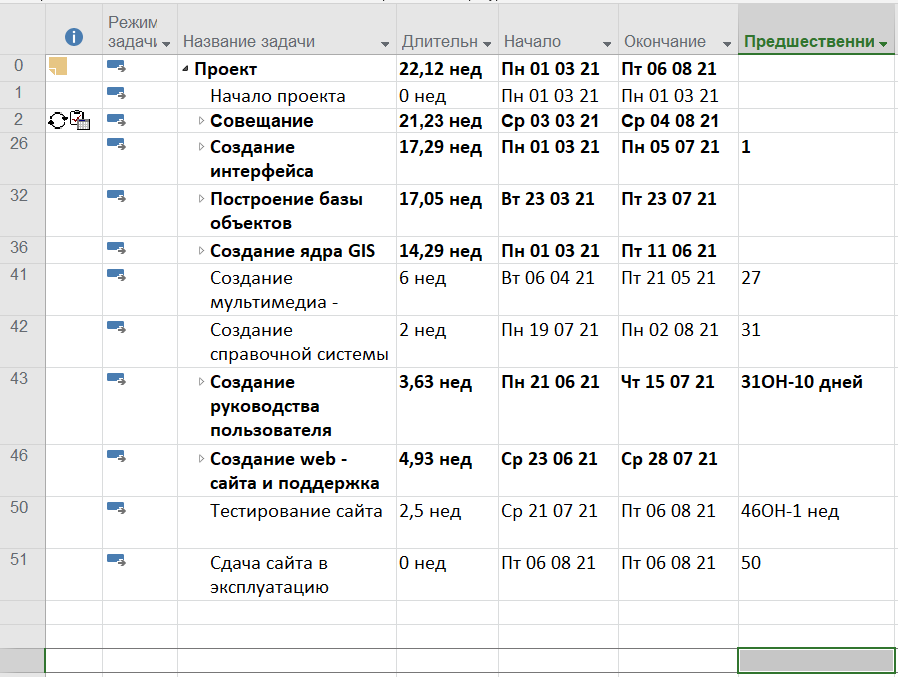
\includegraphics[width=0.7\linewidth]{src/1}
	\caption{Исходный план выполнения}
	\label{fig:1}
\end{figure}

\subsection{Исходная информация о ресурсах}
\begin{figure}[H]
	\centering
	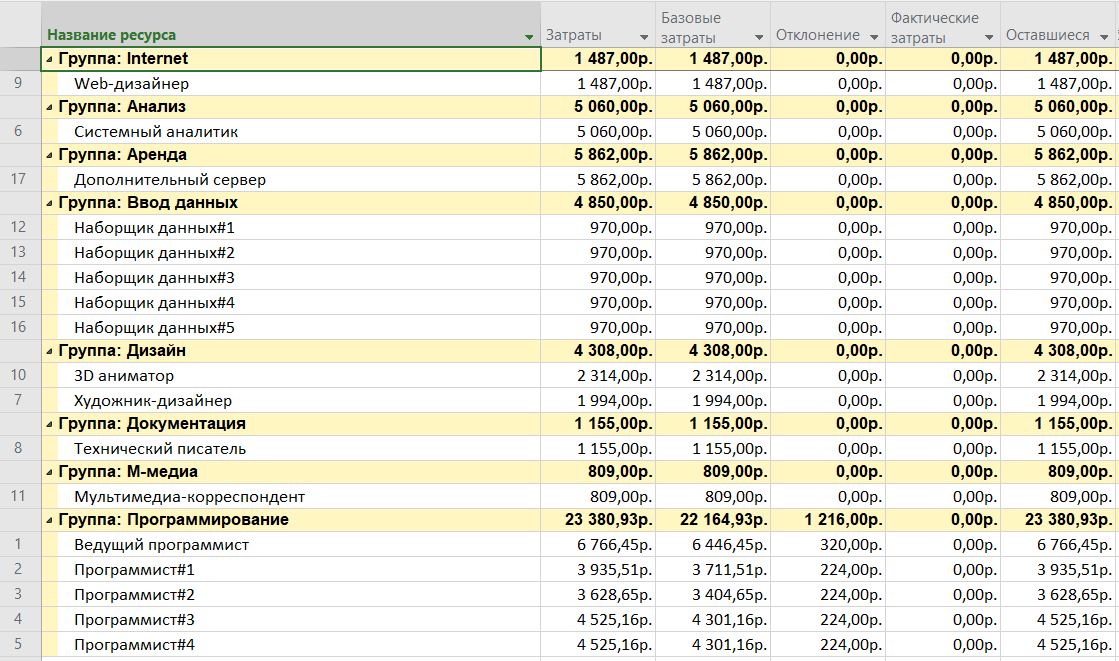
\includegraphics[width=0.7\linewidth]{src/2}
	\caption{Исходные ресурсы}
	\label{fig:2}
\end{figure}

\section{Причины перегрузки ресурсов}
В лабораторной работе №2 наблюдалась перегзку следующих ресурсов:
\begin{enumerate}
	\item Системный аналитик:
	\begin{enumerate}
		\item Анализ и построение структуры базы объектов;
		\item Анализ и проектирование ядра.
	\end{enumerate}
	\item Художник-дизайнер
	\begin{enumerate}
		\item Разработка дизайна руководства;
		\item Разработка дизайна сайта.
	\end{enumerate}
	\item Технический писатель:
	\begin{enumerate}
		\item Написание руководства пользователя;
		\item Создание справочной системы.
	\end{enumerate}
\end{enumerate}

Такая перегузка ресурсов была связана с одновременной работой на занятости 100\% на 2ух задачах.
Способы устрения перегрузок: 
\begin{enumerate}
	\item изменить календарь работы ресурса;
	\item назначить ресурс на неполный рабочий день;
	\item изменить профиль назначения ресурса;
	\item изменить ставку оплаты ресурса;
	\item добавить ресурсу время задерки;
	\item разбить задачу на этапы и перекрыть по времени их выполнения;
	\item автоматическое выравниевание;
\end{enumerate}

Для устранения перегрузки было выбрано "Автоматическое выравнивание"

После авто выравнивания перегрузка ресурсов ушла, но увеличились затраты (С 47500 до 47902).
И продолжительсность проекта возросла до 28 недели, что не удовлетворяет условиям.

\section{Влияние переодических задач на продолжительность и стоимость}

После добавления еженедельного совещания появились следующие проблемы:
\begin{enumerate}
	\item Стоимость проекта увеличилась с 47902р до 67941р. Стоимость проекта увеличилась на 20039р
	\item Появилась перегрузка ресурсов, что логично, по скольку сотрудник не может выполнять задачу и находится на совещании.
	\item Увеличилась продолжительность работ.
\end{enumerate}

Что привело нас к выходу за рамки:
\begin{enumerate}
	\item По времени до 28.68 недель;
	\item По бюджету до 67941р;
\end{enumerate}

\subsection{Оптимизация денежных ресурсов}
Для того что бы снизить траты введем новую ставку на время совещания.
Уберем затраты на использование.
После введния норм затрат на совещание стоимость одного совещания составило 61 рублей.
И того стоимость всех совещаний составило 1769 рублей.
Стоимость проекта с 47902р до 49707р.


\subsection{Оптимизация сроков проекта}
Теперь вернем проект в рамки установленных сроков.
Для этого на разработку модели ядра добавим программиста 2. Длительность проекта уже уменьшилась до 14.09
Добавил еще одного разработчика для создания рабочей версии ядра (программист 3). Срок уменьшился до 31.08.21.
В результате всех оптимазиций:
\begin{enumerate}
	\item Стоимость проект: 47930,14р
	\item Продолжительность: 25,41н 
\end{enumerate}


\section{Задание 1}
Дата отчета: 20.05.21


Запланированный объем (ЗО) - это те средства, которые были бы затрачены на выполнение задачи в период с начала проекта до выбранной даты отчета, если бы задача точно соотвествовала графику и смете. На 20.05.21г ЗО составляет 27 112,61р


Базовая стоимость выполнения работ (БСВР) - это те средства, которые были бы потрачены на выполнение задачи с самого начала проекта, до выбранной даты отчета, если бы фактически выполненная работа оплачивалась согласно смете, т.е. это фактичесое колиетсво рабочих часов, оплачиваемых по сметным ставкам. На 20.05.21г составляет 17 848,25р.


Фактические затраты или фактическая стоимость выполненных работ (ФСВР) - это средства, фактически птраченные на пвыполнение задачи в период с начала проекта до выбранной даты отчета, т. е. это фактическая стоимость задачи или фактическая ставка, умноженная на фактические часы. На 20.05.21г составляет 16 893, 26р (Отклонение от базовой стоимости выполеннных работа составляет 955Р).


Отклонение от календарного плана (ОКП) - сравнивает сметную стоимость плановой и выполненной работы и позволяет вычислить несоответсвие сметы, вызванное исключетельно различиями между плановым и фактическим объемом работы. Для проекта составляет  -9 264р


Отклонение по стоимости (ОКС) - сравнивает сметную и фактическую стоимость выполеннной работы и возволяет выделить нессответсвие сметы, вызванный разницей стоимости ресурсов. Для проекта составляет 955р


Предварительная оценка по завершению (ПОПЗ) - отображает ожидаемые общие затраты для задачи, расчет которых основан на предложении, что оставшиеся часть работы будет выполена в точном соответствии со сметой. ПОПЗ также назывется прогнозом по завершении. Для данного проекта составляет 46 090р


Проект идет  медленне чем планировалось.

\section{Задание 2}
Для того, чтобы отобразить отчет о бюджетной стоимости необходимо открыть во вкладке «Отчеты» пункт меню «Наглядные отчеты».

Исходя из приведенного ниже графика \ref{fig:3} можно сказать, что наибольшие затраты пришлись на 1 неделю 2ого квартала.
\begin{enumerate}
	\item 
\end{enumerate}
\begin{figure}[H]
	\centering
	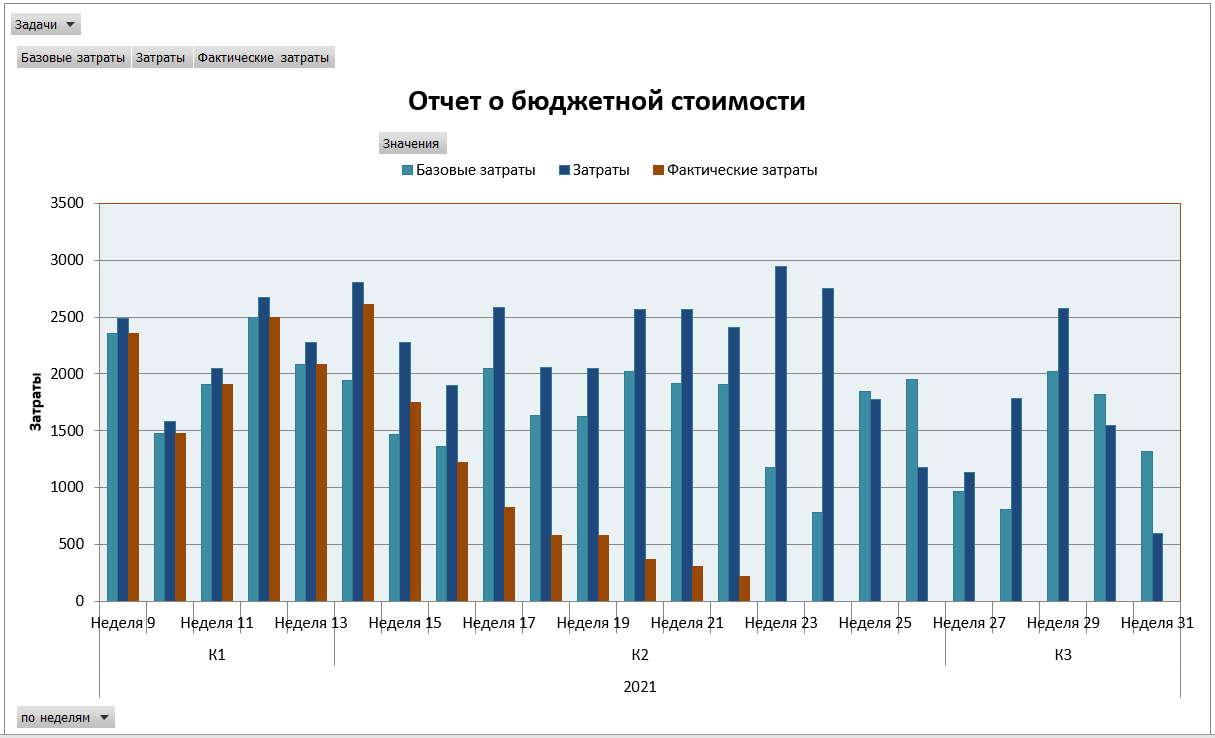
\includegraphics[width=0.7\linewidth]{src/3}
	\caption{График затрат}
	\label{fig:3}
\end{figure}
В это время исполнялись задачи:
\begin{enumerate}
	\item Создание модели ядра;
\end{enumerate}}

Также нам понадобится отчет о превышении затрат по задачам. Для этого во вкладке «Отчеты» необходимо выбрать пункт меню «Затраты», а далее «Превышение затрат» \ref{fig:4}. 
\begin{figure}[H]
	\centering
	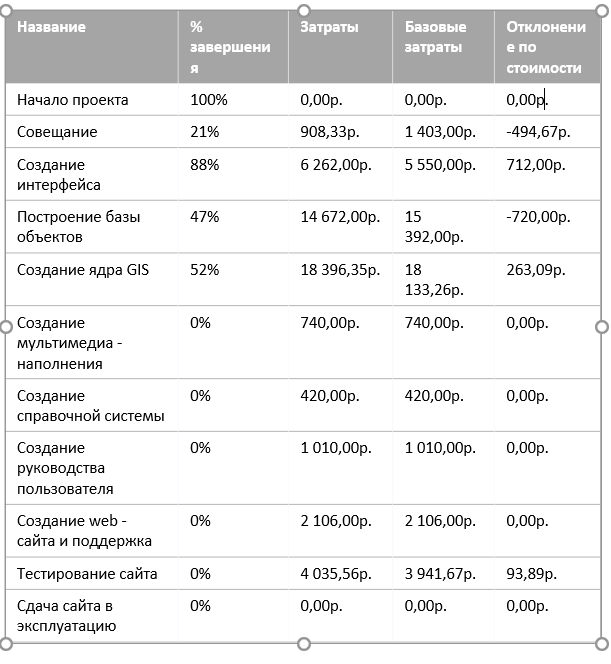
\includegraphics[width=0.7\linewidth]{src/4}
	\caption{Таблица затрат}
	\label{fig:4}
\end{figure}

\section{Задание 3}
Мной было принято решение декомпозировать проект по следующим образом:
\begin{enumerate}
	\item Анализ;
	\item Разработка;
	\item Программирование;
	\item Работа с документацией
	\item Внесение данных;
	\item Тестирование;
	\item Повторяющиеся задачи;
\end{enumerate}

В результате первичной декомпозиции проекта получилось:
\begin{enumerate}
	\item Стоимость 56 694р vs 48 550р.
	\item Продолжительность: 26,83нед. vs 22,11нед.
\end{enumerate}

В результате оптимизации:
\begin{enumerate}
	\item Стоимость: 48 857р
	\item Продолжительность: 20 нед. Дата окончания: 23.07.21
\end{enumerate}

\section{Заключение}
В проекте был проведен анализ базового и фактического плана на 20.04.2021 мая.

У руководителя проекта наибольшая потребность в деньках возникает на 13-14 неделе проекта.
Проведена декомпозиция проекта. В результате удалось сократить проект на 15 дней.
А стоимость увеличилась на 307р.






